\section{Backlog}
\begin{figure}[H]
    \centering
    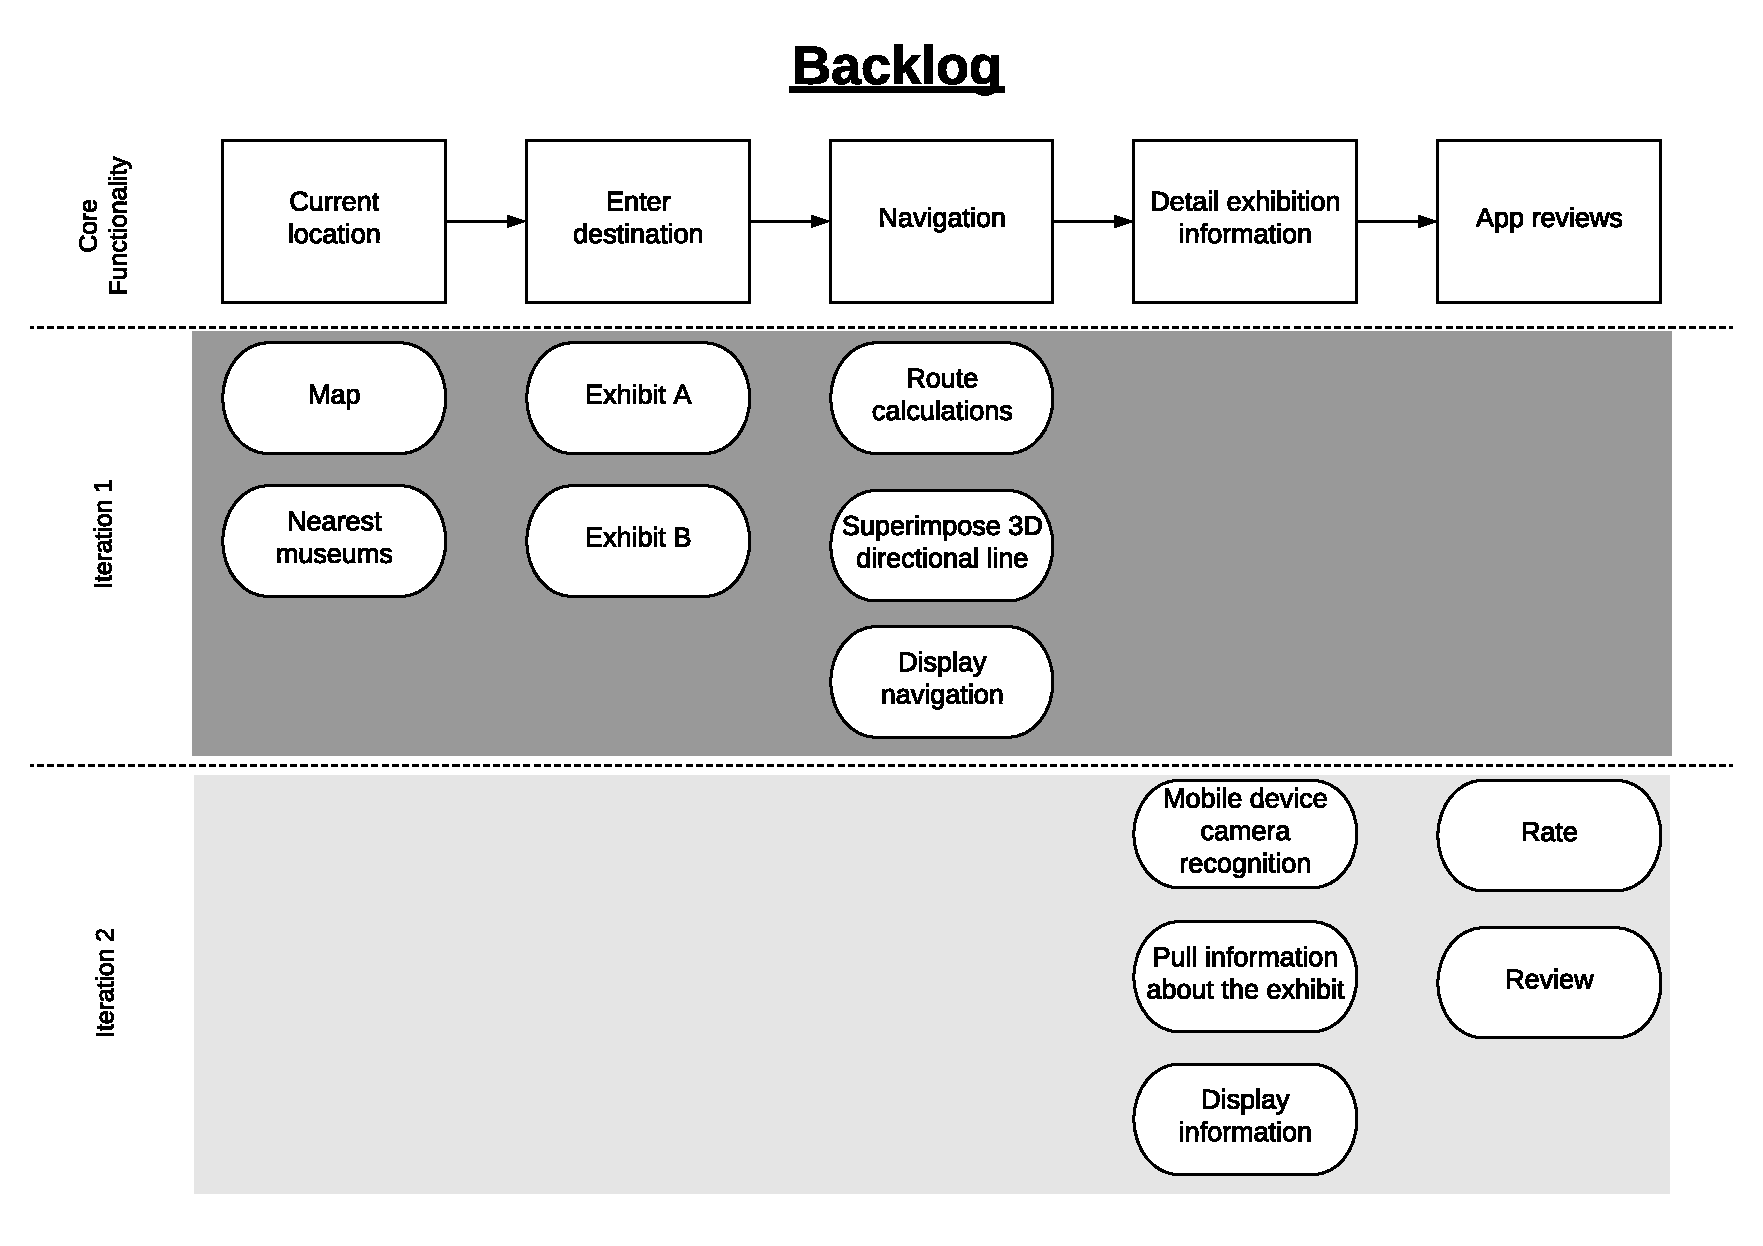
\includegraphics[width=\textwidth]
    {technicalarchitecture/backlog.pdf}
    \caption{Inital Product Backlog}
    \label{fig:productbacklog}
\end{figure}

The product backlog was used as the single source of requirements in order to prioritise releases, and allowed for transparent iteration planning. From the requirements and project scope, each of the five core functionalities were broken down into its major components. Considering the time estimates, the scrum team decided that to demonstrate originality in the project, and to build the base functionalities first, the route calculations and the AR implementation were to form the minimal viable product. Features which required a database such as exhibition item/image recognition, user profiles/logins, and building servers were placed in future releases. These components would take longer than the amount of development time available along with the base functionalities. The team recognised the added time for the construction and integration of a database to the app would increase the risk in not delivering a functional MVP. As a living scrum artifact, the backlog changed accordingly when there were requirements, enhancements, and fixes during the implementation and testing phases of each sprint. In practice, the backlog was maintained on the scrum board hosted on Trello.

% table of time estimates
\begingroup
\renewcommand{\arraystretch}{1.5} % Default value: 1
\begin{table}[H]
\centering
\begin{tabular}{l|c}
\textbf{Function}                & \textbf{Estimate Time (Days)} \\ \hline
Displaying map                   & 0.5                           \\
Finding nearest museums          & 3                             \\
Getting start and end locations  & 5                             \\
Route calculations               & 10                            \\
Superimpose 3D directional line  & 12                            \\
Displaying navigation            & 10                            \\
Mobile device camera recognition & 2                             \\
Retrieve exhibit information     & 10                            \\
Display exhibit information      & 1                             \\
Rating the app                   & 1                             \\
Reviewing the museum visit       & 3                             
\end{tabular}
\caption{Table of time estimates for each function}
\label{table:timeestimates}
\end{table}
\endgroup

\begin{figure}[H]
    \includegraphics[width=\textwidth, height=100mm]
    {sdlc/scrumboard.png}
    \caption{Snapshot of scrum board in action}
    \label{fig:scrumboard}
\end{figure}

\section{Sprint Outlines}
During implementation, four sprints were conducted each lasting one to two weeks. The first sprint lasting one week with the goal of building a beacon for calculating distances between users and objects. The following sprint focused on route calculations; being able to calculate the route between two points in a given space. For the AR part, this was divided into two separate sprints, with the initial one focusing on rendering, and anchoring objects in real-time, and afterwards the integration with all base functionalities.

\section{Front-end}
Front-end development was carried out using Java on Android Studio. 

It was carried out in the early stages of implementation due to the fact that the team had already received user feedback for the UI/UX prototypes. After combining the positive features of the initial design prototypes into one, it became easier to visualise the end result. With aims to create an user interface that is user friendly, and intuitive, various features of the application are self-explanatory. 

As soon as the application is opened, the user is faced with the login page asking for credentials. The user can keep track of their past visits to museums and review various sites; this put in place future developments but not included in the MVP. However, if the user does not have an account they are able to 'Continue as a Guest', and use the services freely without saving any data. When the user has passed the login page, they see the menu.

\begin{figure}[H]
    \centering
    \begin{minipage}[b]{0.4\textwidth}
        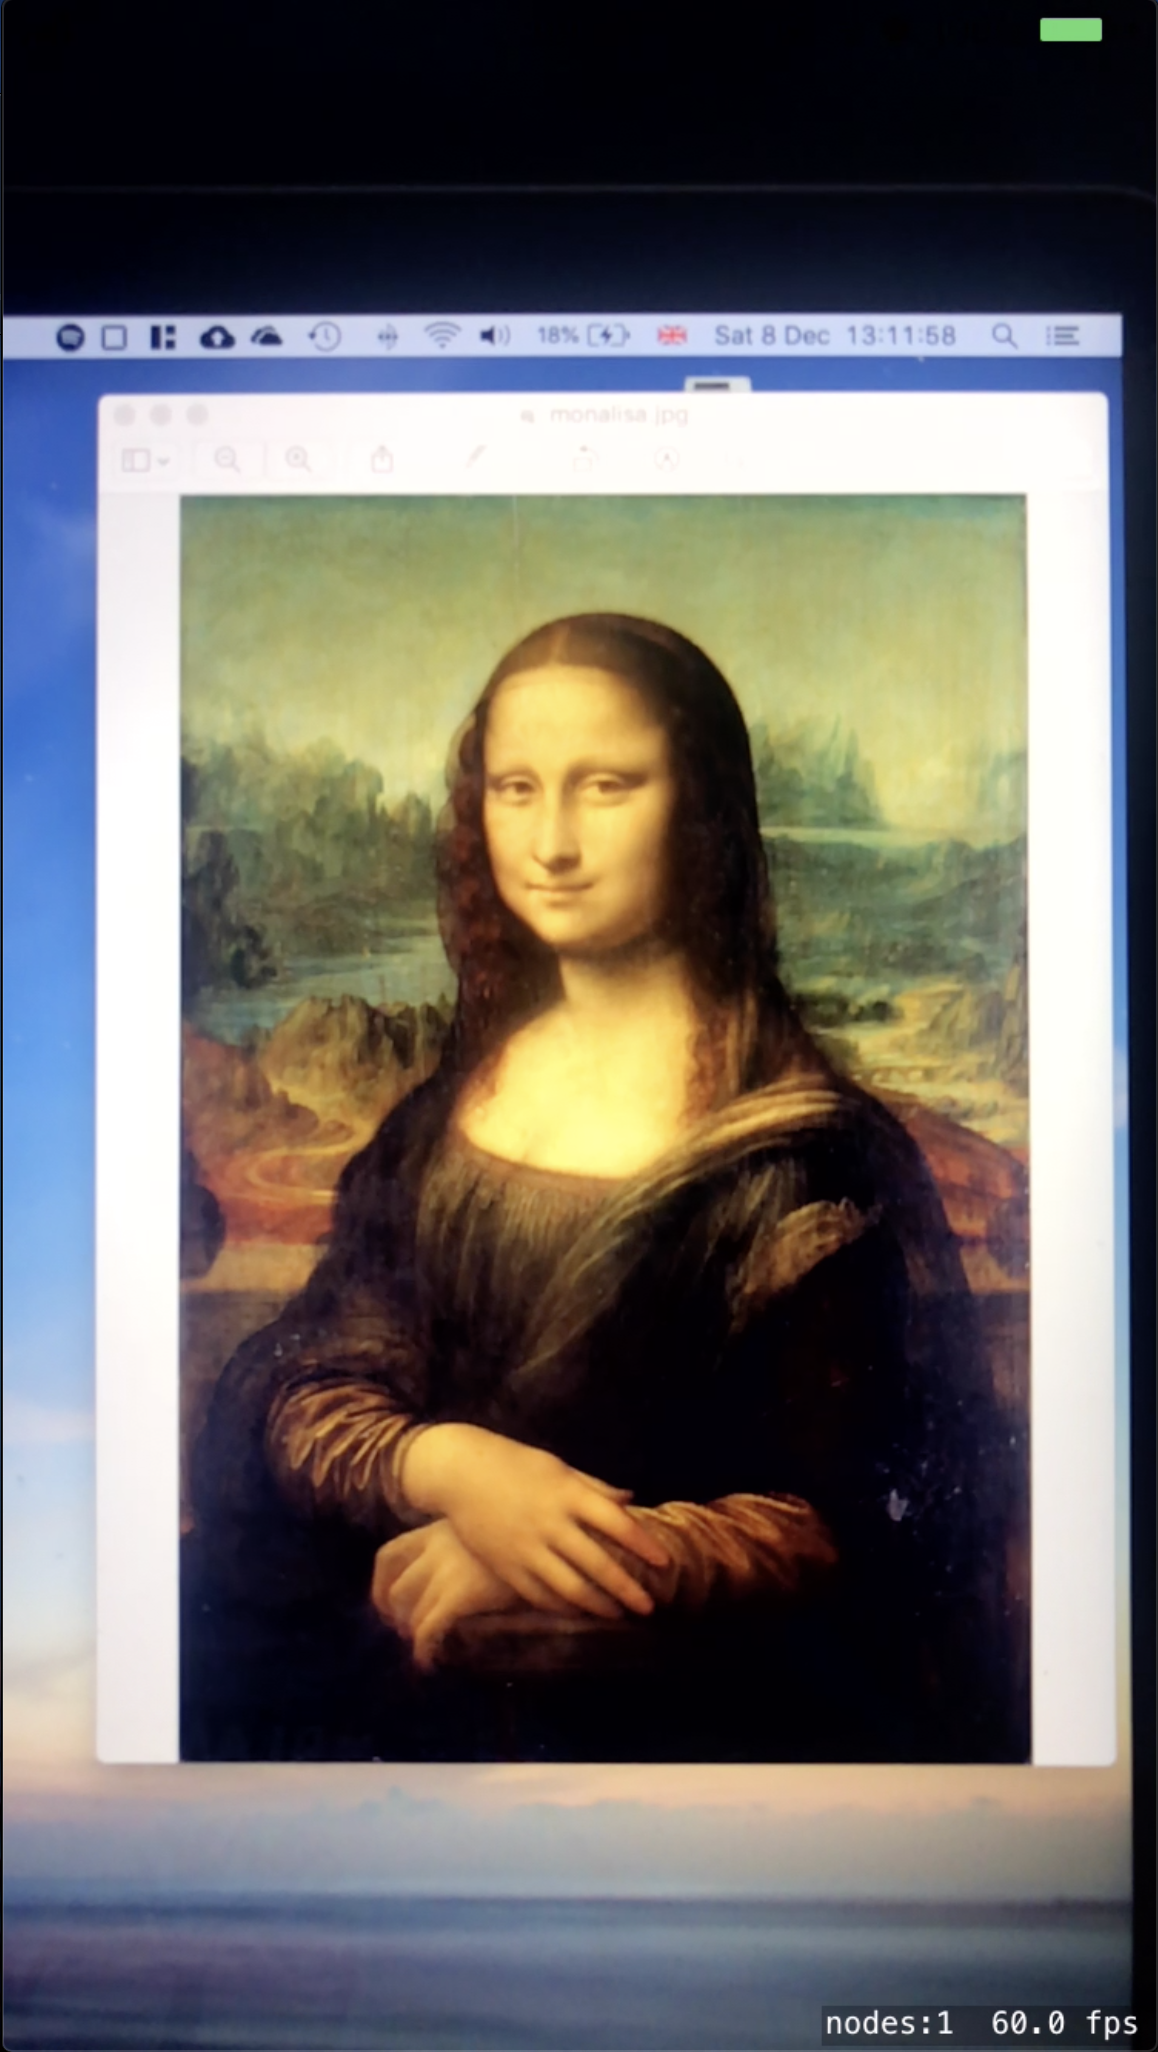
\includegraphics[width=50mm]{prototypes/ui/final/1.png}
        \caption{Log-In Screen}
        \label{fig:loginscreen}
    \end{minipage}
    \qquad
    \begin{minipage}[b]{0.4\textwidth}
        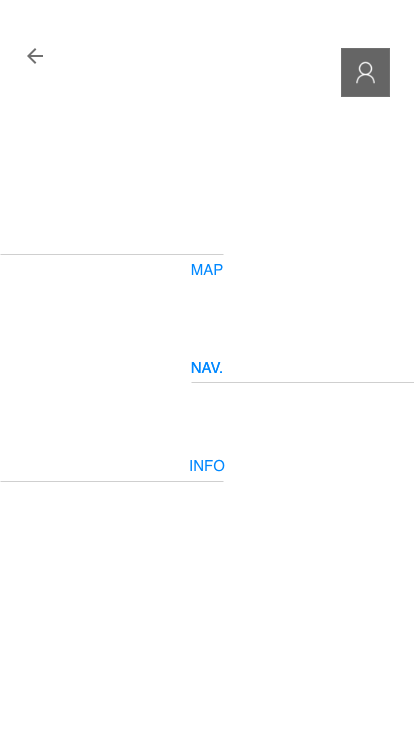
\includegraphics[width=50mm]{prototypes/ui/final/2.png}
        \caption{Menu Screen}
        \label{fig:menuscreen}
    \end{minipage}
\end{figure}

There are three different services that the user can utilise. The 'Map' which shows the user their current location, and surroundings on a 2D map. The 'Nav' menu takes the user to the screen which the user has to then enter their desired destination or exhibit. After all the information has been entered by the user, the user's device displays the AR-enabled camera with the highlighted navigational line directing the user to their destination. However, if the user's device is not compatible with Google's ARCore then the user will not see this screen, and instead faced with an error message. Lastly, the 'info' page will allow the user to see additional information about an exhibit of their choice - this also requires the user to fill out a form.

\lstinputlisting[language=Java, firstline=46, lastline=71, caption=Enabling AR from MenuActivity]{src/MenuActivity.java}

\begin{figure}[H]
    \centering
    \begin{minipage}[b]{0.4\textwidth}
        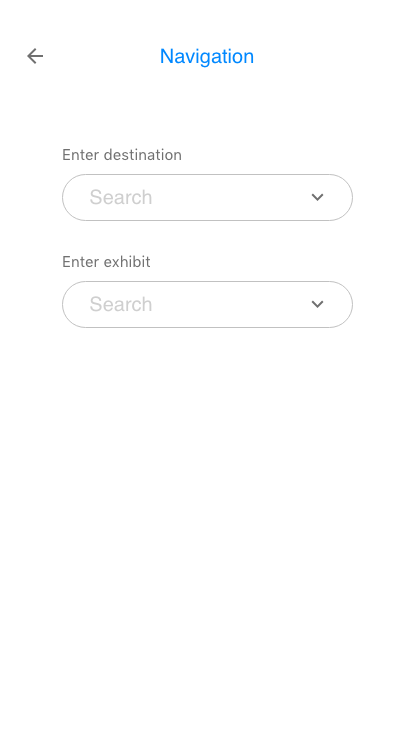
\includegraphics[width=50mm]{prototypes/ui/final/6a.png}
        \caption{Enter Destination}
        \label{fig:enterdestination}
    \end{minipage}
    \qquad
    \begin{minipage}[b]{0.4\textwidth}
        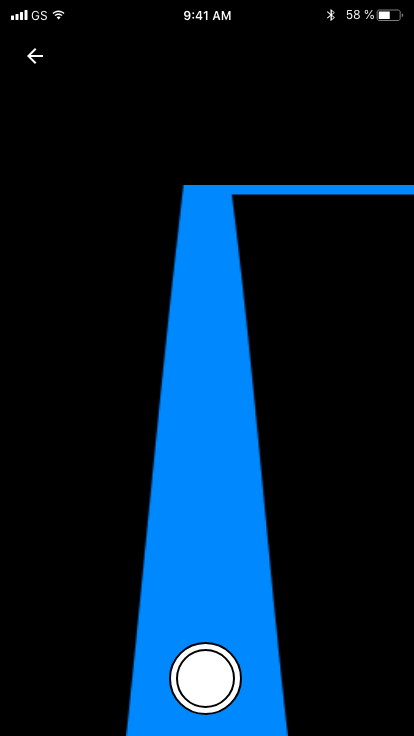
\includegraphics[width=50mm]{prototypes/ui/final/7.png}
        \caption{Navigation Screen}
        \label{fig:navscreen}
    \end{minipage}
\end{figure}

As a result of all the planning and prototyping, when it came to actualising the design in Android Studio it was as simple as writing code for implementation - no further designing was needed, with exception of minor changes such as font sizes.

\begin{figure}[H]
    \centering
    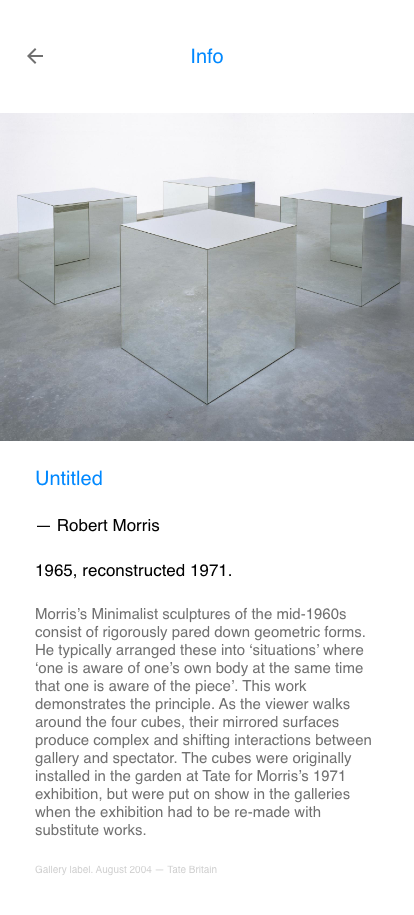
\includegraphics[width=50mm]
    {prototypes/ui/final/8.png}
    \caption{Additional information}
    \label{fig:infoscreen}
\end{figure}

\section{Back-end}
The back-end implementation consisted of developing the application's AR, and route calculations systems, along with integrating, and testing the two constantly throughout the process. Since most of the development team were unfamilar with Android Studio, time over the Christmas vacation was used to gain a firmer understanding of the IDE to reduce the amount of time during implementation to learn basic new skills.

\subsection{Route Calculations}
The scrum team delegated both a sprint, and a consultation with the domain expert in order to ensure this was done correctly.

This concluded in the route calculations using the A* path finding algorithm. Bluetooth was an option in development however, the errors that Bluetooth navigation provided were difficult to handle. Also, the A* algorithm is a better fit for the back-end, since they are both complimentary to augmented reality.

Developed in Kotlin (for development speed), and then converted to Java (to be integrated with the AR segment), the user first enters a destination. That destination becomes a goal node in the context of the route calculations. An attempt to calculate the shortest route using a graph, then outputs that route via the 3D line. As the user traverses that line, their location is constantly updated relative to the goal node so that when the user reaches it, and an alert is shown. It also ensures that the path constantly updates in the case that they ever lose their way.

\subsection{Augmented Reality}
The application's AR research began with the group understanding how Android's ARCore operates with the camera. It was found that the library evaluates the camera's pixels as a set of 2D nodes - it then maps those 2D nodes onto a 3D plane using depth perception \cite{}. This meant that in order to superimpose the 3D line. The output of the route calculations would have to have little, to negligible margin for error. Otherwise, the user could be guided incorrectly.

Once the research was completed, the group delegated a sprint and some research time beforehand to setting up the AR environment that would be utilised by the route calculation system. Therefore, over the sprint, a testing plan was formulated with seven tests to ensure the environment worked in a sound fashion.

\lstinputlisting[language=Java, firstline=93, lastline=115, caption=Creating AR Scene from ARActivity]{src/ARActivity.java}

The AR sceneform (which assists in rendering straightforward 3D scenes without OpenGL) is retreived from the UX XML fragment and the AR Activity fragment. The model is then setup and rendered with an sfb file (the line), and if unrenderable, an exception is thrown. Using the device's camera, when a flat surface is recognised, the object's position is anchored on the device's screen. After, transformable functions are added to the line including qualities such as scale, and position. Finally, the line is then displayed.

\lstinputlisting[language=Java, firstline=117, lastline=126, caption=Setup Model from ARActivity]{src/ARActivity.java}
\lstinputlisting[language=Java, firstline=128, lastline=134, caption=Creating Model from ARActivity]{src/ARActivity.java}

\begin{figure}[H]
    \centering
    \begin{minipage}[b]{0.4\textwidth}
        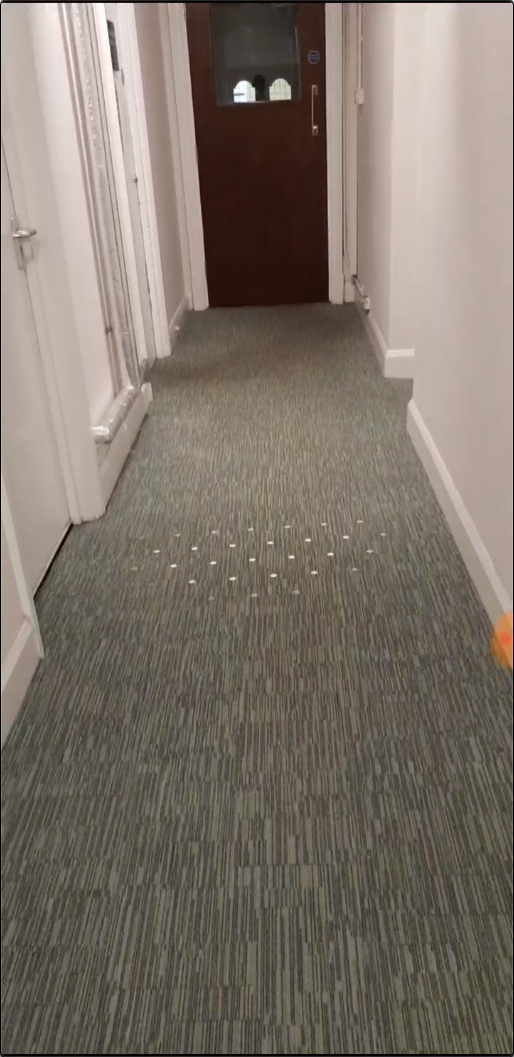
\includegraphics[width=50mm]{final/ar1.png}
        \caption{Detecting flat surface}
        \label{fig:flatsurface}
    \end{minipage}
    \qquad
    \begin{minipage}[b]{0.4\textwidth}
        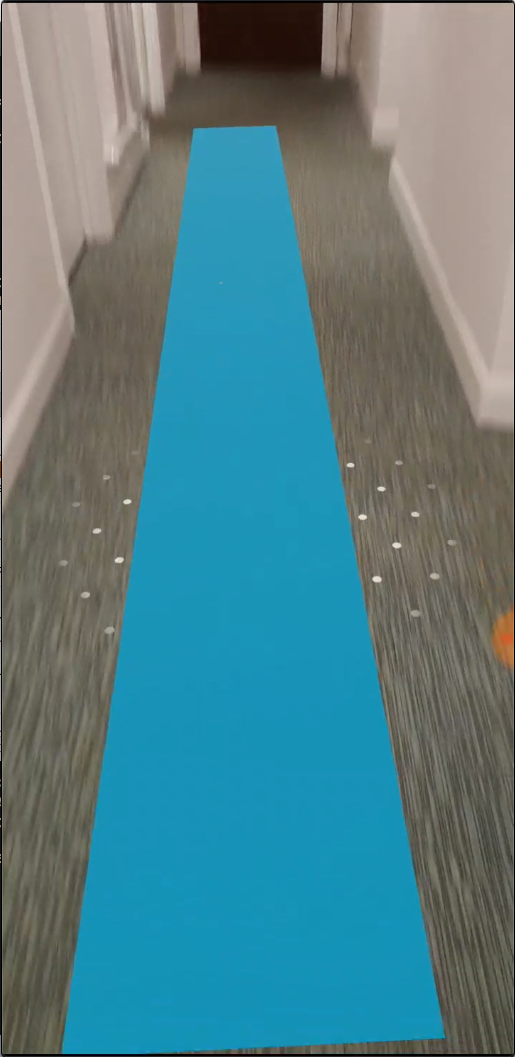
\includegraphics[width=50mm]{final/ar2.png}
        \caption{Anchoring, and displaying straight line object}
        \label{fig:anchor}
    \end{minipage}
\end{figure}

\section{Hardware}
In order to transmit the user’s location to compute a route solution, utilising the Arduino (UNO R3 Mega 2560)’s small foot-print, a simple beacon plan was sought consisting of the Arduino coupled with the Bluetooth HC- 05 RF transceiver. 
 
Figure~\ref{fig:arduino} displays the basic layout of the beacon aside from power input via the board’s USB-B socket. This configuration was able to send the strength of the Bluetooth frequency thereby allowing the computation of a distance.

\begin{figure}[H]
    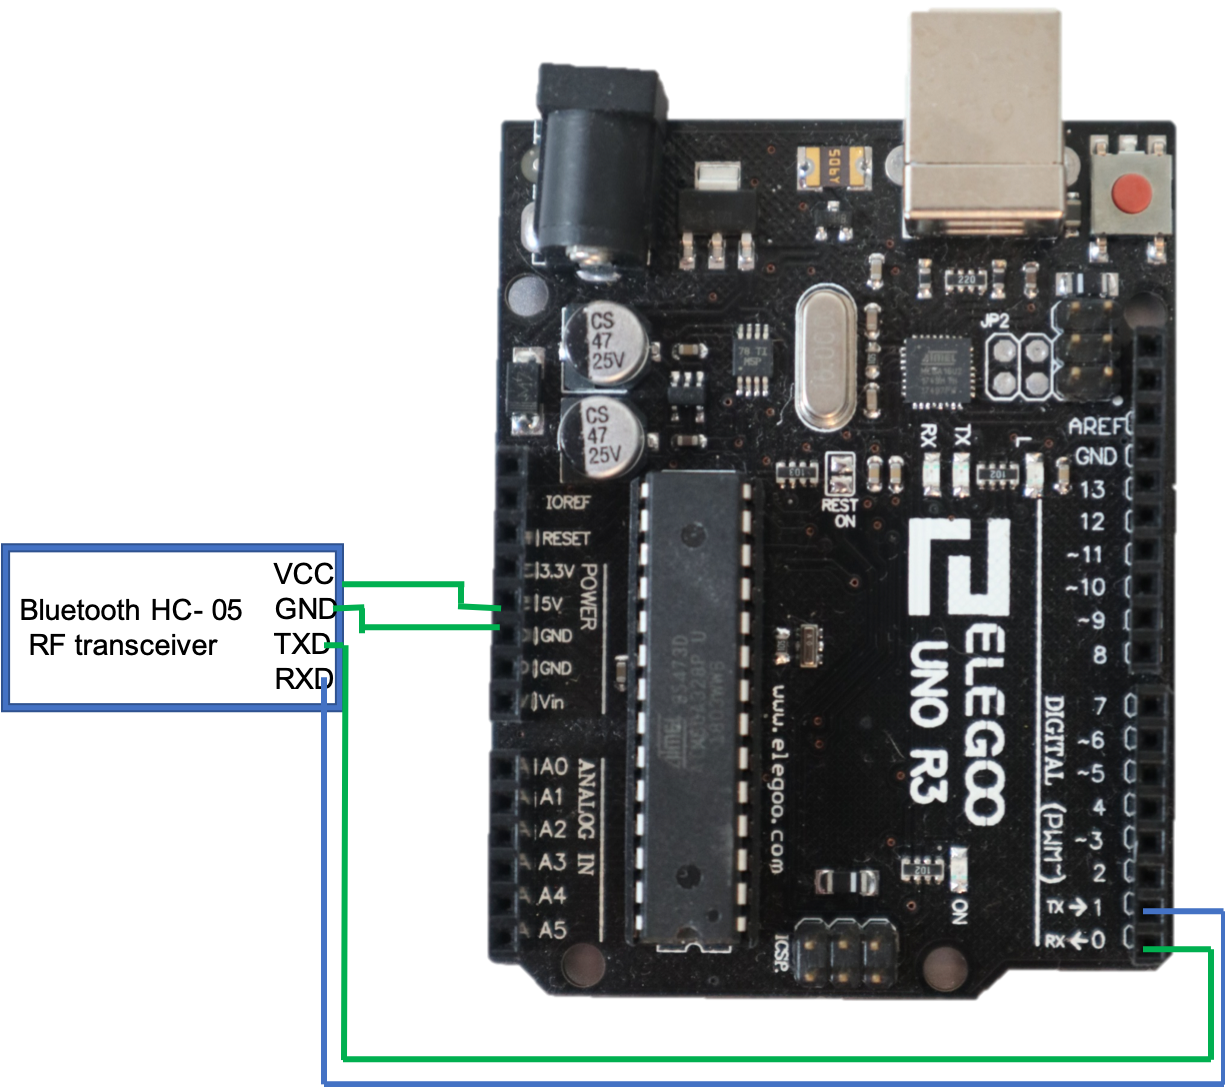
\includegraphics[width=\textwidth, height=100mm]
    {arduino/arduino.png}
    \caption{Arduino layout}
    \label{fig:arduino}
\end{figure}

However, to get more accurate readings, the project would need at least three beacons to demonstrate triangulation wherein three signals are emitted from three angles to get an accurate location. During the testing there was only sufficient means for the procurement of one beacon – this led to an inability to fairly showcase the ideal usage, hindering the projects in this method. 

While it was advised by the domain expert that this Bluetooth solution would be the best policy, it was not practicable given the available resources. In view of these drawbacks, the hardware proposal was ceased. The research provided the team with enough of the methods, and models to pursue a theoretical solution. 

\section{Ethical Audit}
To comply with GDPR, user locations are recorded during the runtime of the application, and upon termination this data is deleted from memory in order to prevent unauthoried access to the user's location. Users are asked initially to give the Bluetooth, camera, and location permissions to use particular functions.

Since the app uses museum maps, and exhibition details, the intellectual property for those will not be under the jurisdiction of the team. Rather, the project members owns the intellectual properties of all technologies that are being created, and used in conjunction with third-party information. Since assigning data and storing details to specific users was not implemented in this iteration, in future versions the app will need to prevent attacks such as SQL injections.

\section{Challenges}
The groups ideas were difficult to manifest due to a lack of technological resources, and a much larger, but relevant issue; the infancy of the AR, and accurate indoor navigation market-places.

Currently, the market relies on Bluetooth technology in order to bypass the problem. However, for this application, using Bluetooth has disadvantages that can prove crucial success to the project. First, the group would have to have access to multiple Arduinos in order to propagate the necessary number of Bluetooth RSSI signals to get an accurate position on the user. Without enough Arduinos, the group would be at risk evaluating the signals inaccurately due to the compromising of the signals by metallic surfaces. Another issue with the Bluetooth technology is the risk that it places the user in. 

The group initialised the solution by finding a prototype that had already existed \cite{smd}. Once found, another challenge arose; the prototype was last maintained in 2016 so the code did not function to begin with. This hurdle was solved by delegating a sprint to the debugging the application.

This halted the software development of the application for a period of time, until the prevailing solution had been devised. A theoretical solution would involve the group hard-coding the geometry of the area to be traversed by the user, and using the coded geospace along with a hard-coded location anchor within that geospace to navigate (A* algorithm with a vector function as the heuristic) the users device.

Finding problems with ARCore library, the group had problems debugging since documentation was vague, and information was scarce. An example of a faced issue was the inability to have the AR section of the application open up on different mobile devices.

A large amount of implementation time was finding usable AR resources, namely the straight line to direct users. Initially, the line file was created, and rendered but did not display on the user's device. To resolve this, a different object file from a GitHub repository was utilised instead. In this case, the line was displayed on the screen, and the group came to resolve that it was an issue to do with the object file, and not sections of the source code.

Further, members of the development team had varying Android versions and SDKs during development, providing inconsistent experiences for each developer. Instead, more pair programming took place so instead of working in an ad-hoc fashion, a collaborative approach was used instead.
